%-------------------------------------------------------------------------------
% This file provides a skeleton ATLAS note.
% \pdfinclusioncopyfonts=1
% This command may be needed in order to get \ell in PDF plots to appear. Found in
% https://tex.stackexchange.com/questions/322010/pdflatex-glyph-undefined-symbols-disappear-from-included-pdf
%-------------------------------------------------------------------------------
% Specify where ATLAS LaTeX style files can be found.
\newcommand*{\ATLASLATEXPATH}{latex/}
% Use this variant if the files are in a central location, e.g. $HOME/texmf.
% \newcommand*{\ATLASLATEXPATH}{}
%-------------------------------------------------------------------------------
\documentclass[NOTE, atlasdraft=true, texlive=2016, UKenglish]{\ATLASLATEXPATH atlasdoc}
% The language of the document must be set: usually UKenglish or USenglish.
% british and american also work!
% Commonly used options:
%  atlasdraft=true|false This document is an ATLAS draft.
%  texlive=YYYY          Specify TeX Live version (2016 is default).
%  coverpage             Create ATLAS draft cover page for collaboration circulation.
%                        See atlas-draft-cover.tex for a list of variables that should be defined.
%  cernpreprint          Create front page for a CERN preprint.
%                        See atlas-preprint-cover.tex for a list of variables that should be defined.
%  NOTE                  The document is an ATLAS note (draft).
%  PAPER                 The document is an ATLAS paper (draft).
%  CONF                  The document is a CONF note (draft).
%  PUB                   The document is a PUB note (draft).
%  BOOK                  The document is of book form, like an LOI or TDR (draft)
%  txfonts=true|false    Use txfonts rather than the default newtx
%  paper=a4|letter       Set paper size to A4 (default) or letter.

%-------------------------------------------------------------------------------
% Extra packages:
\usepackage{\ATLASLATEXPATH atlaspackage}
% Commonly used options:
%  biblatex=true|false   Use biblatex (default) or bibtex for the bibliography.
%  backend=bibtex        Use the bibtex backend rather than biber.
%  subfigure|subfig|subcaption  to use one of these packages for figures in figures.
%  minimal               Minimal set of packages.
%  default               Standard set of packages.
%  full                  Full set of packages.
%-------------------------------------------------------------------------------
% Style file with biblatex options for ATLAS documents.
\usepackage{\ATLASLATEXPATH atlasbiblatex}

% Package for creating list of authors and contributors to the analysis.
\usepackage{\ATLASLATEXPATH atlascontribute}

% Useful macros
\usepackage{\ATLASLATEXPATH atlasphysics}
% See doc/atlas_physics.pdf for a list of the defined symbols.
% Default options are:
%   true:  journal, misc, particle, unit, xref
%   false: BSM, heppparticle, hepprocess, hion, jetetmiss, math, process, other, texmf
% See the package for details on the options.

% Files with references for use with biblatex.
% Note that biber gives an error if it finds empty bib files.
% \addbibresource{ANA-HDBS-2019-04-INT1.bib}
\addbibresource{bib/ATLAS.bib}
\addbibresource{bib/CMS.bib}
\addbibresource{bib/ConfNotes.bib}
\addbibresource{bib/PubNotes.bib}

% Paths for figures - do not forget the / at the end of the directory name.
\graphicspath{{logos/}{figures/}}

% Add you own definitions here (file ANA-HDBS-2019-04-INT1-defs.sty).
\usepackage{ANA-HDBS-2019-04-INT1-defs}

%-------------------------------------------------------------------------------
% Generic document information
%-------------------------------------------------------------------------------

% Title, abstract and document
%-------------------------------------------------------------------------------
% This file contains the title, author and abstract.
% It also contains all relevant document numbers used for an ATLAS note.
%-------------------------------------------------------------------------------

% Title
\AtlasTitle{DiHiggs HH multilepton full Run2}

% Draft version:
% Should be 1.0 for the first circulation, and 2.0 for the second circulation.
% If given, adds draft version on front page, a 'DRAFT' box on top of each other page, 
% and line numbers.
% Comment or remove in final version.
\AtlasVersion{0.1}

% Abstract - % directly after { is important for correct indentation
\AtlasAbstract{%
  This is a bare bones ATLAS document. Put the abstract for the document here.
}

% Author - this does not work with revtex (add it after \begin{document})
\author{The ATLAS Collaboration}

\AtlasAuthorContributor{Merve Nazlim Agaras}{d}{Int. note editor. Group framework developer and coordinator. Fit contact.}
\AtlasAuthorContributor{Xiaohu Sun}{a}{HH -> yy + 2L: MC signal, statistical analysis}
\AtlasAuthorContributor{Abdualazem Fadol}{b}{HH--> yy + 1/2L, HH -->2LSS, object/event selection, software framework}
\AtlasAuthorContributor{Yaquan Fang}{b}{Analysis contact. HH--> yy + 1/2L, HH -->2LSS, object/event selection, software framework}
\AtlasAuthorContributor{Kaili Zhang}{b}{Combination liason. HH--> yy + 1/2L, HH -->2LSS, object/event selection, software framework}
\AtlasAuthorContributor{Djamel Eddine Boumediene}{d}{QMisID DD estimates. Supervisor of Merve Nazlim Agaras.}
\AtlasAuthorContributor{Maosen Zhou}{b}{HH--> yy + 1/2L, HH -->2LSS, object/event selection, software framework}
\AtlasAuthorContributor{Weiming Yao}{c}{HH -> 1L + jets / 2had taus + jets: Tau selection and fakes}
\AtlasAuthorContributor{Rohin Narayan}{e}{HH -> 2L/3L: Fake leptons, kinematic discriminants, software framework} 
\AtlasAuthorContributor{Allison McCarn Deiana}{e}{HH -> 2L/3L: Fake leptons, kinematic discriminants, software framework}
\AtlasAuthorContributor{Xingguo Li}{f}{HH -> 2/3L + jets}
\AtlasAuthorContributor{Chihao Li}{g}{HH -> 4L + 2b: MC generation, object definition, event selection, combination}
\AtlasAuthorContributor{Yusheng Wu}{g}{HH -> 4L + 2b: MC generation, object definition, event selection, combination}
\AtlasAuthorContributor{Bartlomiej Zabinski}{h}{HH -> taus + X: Tau optimisation, machine learning, fit, framework}
\AtlasAuthorContributor{Anna Kaczmarska}{h}{HH -> taus + X: Tau optimisation, machine learning, fit, framework}
%\AtlasAuthorContributor{Ana Elena Dumitriu}{j, i}{Support in group framework 1.} Tiesheng Dai, Hang Qi, Bing Li, Bing Zhou
\AtlasAuthorContributor{Tiesheng Dai}{i}{HH -> 4L + 2b: MC signal, object definition, event selection, interpretation, combination}
\AtlasAuthorContributor{Hang Qi}{i}{HH -> 4L + 2b: MC signal, object definition, event selection, interpretation, combination}
\AtlasAuthorContributor{Bing Zhou}{i}{HH -> 4L + 2b: MC signal, object definition, event selection, interpretation, combination}
\AtlasAuthorContributor{Huirun Chen}{j}{HH->1L+3tau had: MC signal production, truth studies}
\AtlasAuthorContributor{Xiaozhong Huang}{j}{HH->1L+3tau had: MC signal production, truth studies}
\AtlasAuthorContributor{Bowen Zhang}{j}{HH->1L+3tau had: MC signal production, truth studies}
\AtlasAuthorContributor{Lei Zhang}{j}{HH->1L+3tau had: MC signal production, truth studies}
\AtlasAuthorContributor{Liang Li}{k}{HH -> 2/3L + jets}
\AtlasAuthorContributor{Jiannan Tang}{k}{HH -> 2/3L + jets}
\AtlasAuthorContributor{Lebohang Mokoena}{l}{X -> SH -> 2L + jets: MC signal, event selection, bkg estimation, statistical analysis}
\AtlasAuthorContributor{Bruce Mellado}{l}{X -> SH -> 2L + jets: MC signal, event selection, bkg estimation, statistical analysis}
\AtlasAuthorContributor{Lehumo Mashishi}{l}{X -> SH -> 2L + jets: MC signal, event selection, bkg estimation, statistical analysis}
\AtlasAuthorContributor{Jeremiah Kgomotso Monnakgotla}{l}{X -> SH -> 2L + jets: MC signal, event selection, bkg estimation, statistical analysis}
%\AtlasAuthorContributor{Dylan Kisliuk}{f}{Tau fake estimates.}
\AtlasAuthorContributor{Yesenia Hernandez}{l}{Analysis contact. X -> SH -> 2L + jets: MC signal, event selection, bkg estimation, statistical analysis}

\affil[a]{Manchester}
\affil[b]{Beijing IHEP	}
\affil[c]{Berkeley LBNL	}
\affil[d]{LPC Clermont-Ferrand}
\affil[e]{Dallas SMU}
\affil[f]{DESY}
\affil[g]{USTC}
\affil[h]{Krakow IFJ PAN}
\affil[i]{Michigan}
\affil[j]{Nanjing}
\affil[k]{Shanghai}
\affil[l]{Witwatersrand}






% Authors and list of contributors to the analysis
% \AtlasAuthorContributor also adds the name to the author list
% Include package latex/atlascontribute to use this
% Use authblk package if there are multiple authors, which is included by latex/atlascontribute
% \usepackage{authblk}
% Use the following 3 lines to have all institutes on one line
% \makeatletter
% \renewcommand\AB@affilsepx{, \protect\Affilfont}
% \makeatother
% \renewcommand\Authands{, } % avoid ``. and'' for last author
% \renewcommand\Affilfont{\itshape\small} % affiliation formatting
% \AtlasAuthorContributor{First AtlasAuthorContributor}{a}{Author's contribution.}
% \AtlasAuthorContributor{Second AtlasAuthorContributor}{b}{Author's contribution.}
% \AtlasAuthorContributor{Third AtlasAuthorContributor}{a}{Author's contribution.}
% \AtlasContributor{Fourth AtlasContributor}{Contribution to the analysis.}
% \author[a]{First Author}
% \author[a]{Second Author}
% \author[b]{Third Author}
% \affil[a]{One Institution}
% \affil[b]{Another Institution}


% If a special author list should be indicated via a link use the following code:
% Include the two lines below if you do not use atlasstyle:
% \usepackage[marginal,hang]{footmisc}
% \setlength{\footnotemargin}{0.5em}
% Use the following lines in all cases:
% \usepackage{authblk}
% \author{The ATLAS Collaboration%
% \thanks{The full author list can be found at:\newline
%   \url{https://atlas.web.cern.ch/Atlas/PUBNOTES/ATL-PHYS-PUB-2016-007/authorlist.pdf}}
% }

% ATLAS reference code, to help ATLAS members to locate the paper
\AtlasRefCode{ANA-HDBS-2019-04}

% ATLAS note number. Can be an COM, INT, PUB or CONF note
\AtlasNote{ANA-HDBS-2019-04-INT1}

% Author and title for the PDF file
\hypersetup{pdftitle={ATLAS document},pdfauthor={The ATLAS Collaboration}}
\usepackage{multirow}

%-------------------------------------------------------------------------------
% Content
%-------------------------------------------------------------------------------
\begin{document}

\maketitle

\tableofcontents

% List of contributors - print here or after the Bibliography.
\PrintAtlasContribute{0.30}
%\clearpage

% Tex for mainbody
\clearpage
%\input{Tex/Status.tex}
\clearpage
\section{Introduction}
\label{sec:intro}

With the discovery of a new scalar particle the Higgs boson~\cite{HIGG-2012-27,CMS-HIG-12-028} at the LHC~\cite{Evans:2008zzb} by the ATLAS and CMS collaborations with a mass of 125 GeV~\cite{HIGG-2016-33,HIGG-2013-12,HIGG-2014-14,CMS-HIG-14-009}, the whole content of the Standard Model (SM) of particle physics became complete. A priority of the ATLAS and CMS collaborations has been to better understand its properties and couplings.
After the EWSB and the higgs field acquires the vev, the higgs potential obtained in Equation.. can be obtained as following:
\begin{align}
	V(\phi) \rightarrow V(\phi)_{\text{EWSB}} =  -\lambda \nu^2 h^2 - \lambda \nu h^3 - \frac{1}{4} \lambda h^4 + \text{const.}
	\label{eq:higgs_pot}
\end{align}
The first term of the above equation is the Higgs mass term, and the remaining are the trilinear and quadri-linear Higgs-self couplings,
\begin{align}
	\underbrace{m_{h} = \sqrt{ - 2 \mu^2} = \sqrt{ 2 \lambda v^2 }}_\text{Higgs boson mass} \hspace{1cm} \underbrace{\lambda_{hhh} \propto \frac{m_h^2}{v} \hspace{1cm} \lambda_{hhhh} \propto \frac{m_h^2}{v^2}}_\text{Trilinear and quadri-linear Higgs self-couplings}.
	\label{eq:higgs_self_couplings}
\end{align}
A measurements of this couplings would therefore give a hint about the actual structure of the potential, whose shape can have  theoretical consequences. The quartic Higgs coupling, $\lambda_{hhhh}$, can not be measured at LHC since the cross-section of triple Higgs production is small~\cite{PhysRevD.74.113008}~\cite{PhysRevD.93.035026}, while the trilinear coupling can be probed directly in Higgs pair production. 

The trilinear coupling leads to non-resonant pair production of Higgs bosons, where an off-shell
Higgs decays to a pair of Higgs bosons, the leading production mechanism being $gg$-fusion.
Direct observation of Higgs pair production would lead to measurements directly sensitive to
$\lambda$ but in the SM there are competing diagrams, proceeding via quark (re: top quark) loops
that are instead senstive to the Yukawa coupling of the Higgs rather than the trilinear coupling
$\lambda$. These \dihiggs production mechanisms are illustrated in the Feynman diagrams presented
in Figure \ref{fig:sm_nonres_hh}. Not only does the quark-loop induced process present
itself as an irreducible background to the process senstive to the Higgs self-coupling, but
it interfereces \textit{destructively} with the latter, making the observation of this
type of Higgs pair production more challenging.


% Due to its lower cross section, diHiggs production is not expected to be observed in the current data taking setup, however it is possible to define limits on the measurement to constrain the BSM physics theories. 
\begin{figure}[!htb]
    \centering
    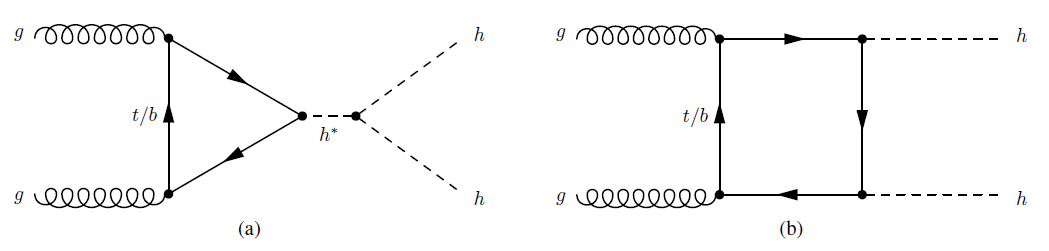
\includegraphics[width=0.9\textwidth]{figures/sm_nonres_hh_production}
    \caption{Representative diagrams that contribute to non-resonant \hh production.
    \textit{Left}: Diagram that is sensitive to the trilinear coupling, $\lambda$.
    \textit{Right}: Box diagram that interferese destructively with the $\lambda$-sensitive
    process.} 
    \label{fig:sm_nonres_hh}
\end{figure}


As a result of the destructive interference, and the already relatively large Higgs mass of
125 \GeV, the SM \dihiggs production has a total cross-section of $\sim 33.4$ fb ~\cite{CERN-YR-4}
at a \pp center-of-mass collision energy of 13 \TeV. The inclusive cross-section for the pair-production
of top quarks, which will be one of the dominant SM backgrounds in the present
analysis, is nearly 1000 pb, or $1\times10^6$ fb ~\cite{TOPQ-2015-09, ATLAS-CONF-2015-049}. That
of \textit{single} Higgs production is $\sim 50$ pb, or $5 \times 10^4$ fb ~\cite{ATLAS-CONF-2015-060}.

Furthermore, enhancements to the di-Higgs production rate, either non-resonantly or through a resonance, may be observable with the full Run2 dataset and would point to new physics beyond the Standard Model, making such analyses interesting now. The wide class of two Higgs double models (2HDM) predict an altered and enlarged
Higgs sector from which the currently Higgs is built.
The Minimal Supersymmetric Standard Model
(MSSM) is a  class of 2HDM. For the latter set, one such model is a Randall-Sundrum
type graviton or the lightest Kaluza-Klein excitation which have masses of at least
$2\times$ the mass of the SM Higgs boson. The presence of such BSM scenarios would act to alter
the measured value of $\lambda$ with respect to that of the SM, potentially enlarging it.
As a result, early evidence for the pair-production of Higgs bosons within the current
Run-2 dataset may indicate the presence of new physics without having to resort to
precision measurements of $\lambda$. Examples of such decay
scenarios are illustrated in example Feynman diagrams in Figure \ref{fig:2hdm_feynman_diagrams}.

\begin{figure}[!htb]
    \centering
    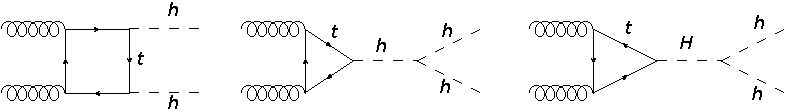
\includegraphics[width=0.8\textwidth]{figures/mg5_hh_heavy_scalar.png}
    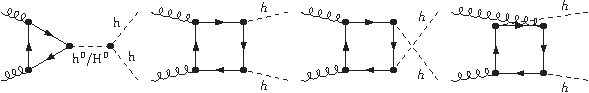
\includegraphics[width=0.8\textwidth]{figures/mg5_hh_2hdm_cp_even.png}
    \caption
    {
        Diagrams contributing to enhanced $hh$ production scenarios.
        \textit{Top}: A heavy scalar, $H$, that couples to the Standard Model Higgs
        boson, $h$, contributes to the Standard Model processes (left two diagrams).
        \textit{Bottom}: CP-even diagrams in 2HDM scenario that contribute to enhanced
        non-resonant production of Standard Model Higgs bosons as well as resonant
        channels with the heavy CP-even Higgs, $H^0$, decaying to the Standard Model
        low-mass CP-even Higgs, $h$.
    }
    \label{fig:2hdm_feynman_diagrams}
\end{figure}


In addition to the hh production mechanisms described above, the searches for evidence of an dditional extended Higgs sector model that introduces two new heavy Higgs bosons, X and S~\cite{vonBuddenbrock:2016rmr}. In this model, $X$ couples strongly to both $S$ and $h$. $S$ couples weakly to SM particles, suppressing direct production, but has the same mass-dependent branching ratios as $h$. 

Searches for resonant Higgs pair production have been performed in a number of final states, $b\bar{b}b\bar{b}$, $b\bar{b}\tau^{\pm}\tau^{\mp}$, $b\bar{b}\gamma\gamma$, $W^{\pm}W^{\mp *}\gamma\gamma$, $b\bar{b}VV$ (With $V$ either $Z$ or $W$) and $W^+W^-W^+W^-$ at $\sqrt{s}=8\,\TeV$ and $\sqrt{s}=13\,\TeV$ by ATLAS~\cite{HIGG-2013-33,Aad:2019uzh} and CMS collaborations~\cite{CMS-HIG-13-032,CMS-HIG-15-013,PhysRevLett.122.121803} including the combination of multiple final states. 

In this note, the searches for the \dihiggs non-resonant production in multilepton final states is described. Typically the decay modes of \dihiggs of $W^+W^-W^+W^-$, $ZZ^*bb$, $VV\tauh\tauh$, $\tauh\tauh\tauh\tauh$, $ZZZZ$ are the dominant ones which corresponds to 5.7\% of all \dihiggs decays. Additionally, $\gamma\gamma + X$ final states are studied which corresponds to 0.13\% of \dihiggs decays. Simple extension of the SM by introducing two new scalars $gg \rightarrow X \rightarrow SH$ signature is investigated.


This note is organised as follows: Section~\ref{sec:dataset} describes the Monte Carlo (MC) samples as well as the 
recorded dataset used in this analysis. The object definition and event preselection are detailed in Section~\ref{sec:objselec}. 
The signal region definitions and the multivariate analysis discriminants are described in Section~\ref{sec:eventselec}. 
The reducible background estimates using data-driven method are explained in Section~\ref{sec:nonpromptbkg}. 
%Section~\ref{sec:bkgval} shows the data and MC agreement of the prompt lepton background contributions in 
various validation regions.  
Theoretical and experimental systematic uncertainties are described in Section~\ref{sec:systematics}. 
An overview of the signal regions before the fit can be found in Section~\ref{sec:signalregion}.
Section~\ref{sec:results} describes the expected fit results for each individual channel and the 
expected and observed fit results for the combination. 
Finally, the conclusions are summarised in Section~\ref{sec:conclusion}.




\clearpage
\section{Data and Monte Carlo samples}
\label{sec:dataset}
This analysis uses 139~fb$^{-1}$ of data collected from proton-proton collision recorded by the ATLAS 
detector at $\sqrt{s}=13$ TeV during 2015-2018. The data set has been collected with a 
bunch crossing of 25 ns, IBL on, and verifying data quality cuts namely which must be in the
recommended Good Run List.
%\footnote{For 2015 dataset:
%\textit{data15\_13TeV.periodAllYear\_DetStatus-v79-repro20-02\_DQDefects-00-02-02\_PHYS\_StandardGRL\_All\_Good\_25ns.xml};
%for 2016 dataset: 
%\textit{data16\_13TeV.periodAllYear\_DetStatus-v88-pro20-21\_DQDefects-00-02-04\_PHYS\_StandardGRL\_All\_Good\_25ns.xml} \\}.  

The analysis uses data being prepared with \verb|xAOD| format and further produced to \verb|DxAOD| 
format using \verb|HIGG8D1| derivation framework. This \verb|xAOD| to \verb|DxAOD| derivation 
provides a reduction specifically for the \tth events with multileptons in the final states. 
The total size of data set has been reduced to 3.6 \% for simulated \ttbar 
events and 0.1\% for collision data set. The size reduction is the result of applying 
smart slimming (remove un-needed variables), thinning (remove entire objects from events) and 
additional skimming on both collision dataset and MC samples. The skimming in \verb|HIGG8D1| derivations consists of removing an event if 
it does not fulfil the following selection: 
\begin{itemize}
  \item at least two light leptons passing loose identification criteria with leading lepton $p_{T}>$ 15 GeV and subleading
  lepton $p_{T}>$ 5GeV, within $|\eta|<$ 2.6
  \item at least one light lepton passing loose identification criteria with $p_{T}>$ 15 GeV and $|\eta|<$ 2.6, and at least
  two hadronic taus. The tau lepton has to pass \verb|JetBDTSigLoose| requirement with $p_{T}>$ 15 GeV, its charge must be
  one and it must have one or three associated tracks.
\end{itemize}

\subsection{Monte Carlo samples}
\label{subsec:ms}

\begin{table}
\begin{center}
{\small
\setlength\tabcolsep{1.5pt}
\begin{tabular}{llllll}
\hline\hline
Process & Generator & Parton Shower & PDF & Tune  \\
& (alternative) & (alternative) & & \\
\hline
\ttH & \textsc{Powheg-BOX} \cite{powhegtt}  & \textsc{Pythia} 8\ & NNPDF 3.0 NLO \cite{Ball:2014uwa}/ & A14 \\
     &                                         &                                       & NNPDF 2.3 LO \cite{Ball:2012cx} \\
     & (-) & (\textsc{Herwig++}) &  \\
$tHqb$ & \textsc{MG5\_aMC} & \textsc{Pythia} 8 & CT10 \cite{ct10} & A14  & \\
$tHW$ & \textsc{MG5\_aMC} & \textsc{Herwig++}  & CT10 & UE-EE-5   \cite{Seymour:2013qka}   \\
& & & /CTEQ6L1 \cite{cteq6l1,cteq6}  \\
%$\ttbar W$ & \textsc{MG5\_aMC} & \textsc{Pythia} 8 & NNPDF 3.0 NLO & A14   \\
%& & & /2.3 LO \\
$\ttbar W$ & \textsc{Sherpa 2.2.1}~\cite{sherpa} & \textsc{Sherpa 2.2.1}  & NNPDF 3.0 NNLO  & \textsc{Sherpa} default   \\
& (\textsc{MG5\_aMC}) & (\textsc{Pythia} 8) &  \\
$\ttbar (Z/\gamma^*)$ & \textsc{MG5\_aMC} & \textsc{Pythia} 8 & NNPDF 3.0 NLO & A14  \\
&&& /2.3 LO \\
& (\textsc{Sherpa}) & (\textsc{Sherpa}) &  \\
$t (Z/\gamma^*)$ & \textsc{MG5\_aMC} & \textsc{Pythia} 8  & CTEQ6L1 & Perugia2012 \cite{perugia}  \\
$t W (Z/\gamma^*)$ & \textsc{MG5\_aMC} & \textsc{Pythia} 8 & NNPDF 2.3 LO  & A14  \\
$t\bar t t$, $t\bar t t\bar t$ & \textsc{MG5\_aMC} & \textsc{Pythia} 8 & NNPDF 2.3 LO & A14 \\
$t\bar t W^+ W^-$ & \textsc{MG5\_aMC} & \textsc{Pythia} 8 & NNPDF 2.3 LO & A14  \\
$\ttbar$ & \textsc{Powheg-BOX} \cite{powhegtt} & \textsc{Pythia} 8 & CT10/CTEQ6L1 & Perugia2012  \\
$\ttbar\gamma$ & \textsc{MG5\_aMC} & \textsc{Pythia} 8 & NNPDF 2.3 LO & A14  \\
$s$-, $t$-channel, & \textsc{Powheg-BOX} \cite{powhegstp,powhegstp2} & \textsc{Pythia} 6 & CT10 & Perugia2012   \\
 $Wt$ single top & & & /CTEQ6L1 \\
$VV$, $qqVV$, & \textsc{Sherpa} 2.2.2 \cite{sherpa} & \textsc{Sherpa} & NNPDF 3.0 NNLO & \textsc{Sherpa} default  \\
$VVV$ & & & \\
$Z \to \ell^+\ell^-$ & \textsc{Sherpa} 2.2 & \textsc{Sherpa} & NNPDF 3.0 NLO & \textsc{Sherpa} default \\
%$W \to \ell\nu$ & \textsc{Sherpa} & \textsc{Sherpa} & CT10 & \textsc{Sherpa} default \\
\hline\hline
\end{tabular}
}
\caption{\label{tab:mcconfig} The configurations used for event generation of signal and background processes. 
If only one parton distribution function (PDF) is shown, the same one is used for both the matrix element (ME) and parton shower generators; 
if two are shown, the first is used for the matrix element calculation and the second for the parton shower.  ``V'' refers to production of 
an electroweak boson ($W$ or $Z/\gamma^*$).  ``Tune'' refers to the underlying-event tune of the parton shower generator. ``\textsc{MG5\_aMC}'' 
refers to \textsc{MadGraph5\_aMC@NLO} 2.2.1~\cite{Alwall:2014hca}; ``\textsc{Pythia} 6'' refers to version 6.427~\cite{Pythia6}; ``\textsc{Pythia} 8'' 
refers to version 8.2~\cite{Pythia8}; ``\textsc{Herwig++}'' refers to version 2.7~\cite{Bahr:2008pv}.  Samples using \textsc{Pythia} 6 or \textsc{Pythia} 8  
have heavy flavour hadron decays modelled by \textsc{EvtGen} 1.2.0~\cite{Lange:2001uf}.  All samples include leading-logarithm photon emission, either modelled 
by the parton shower generator or by \textsc{PHOTOS}~\cite{Golonka:2005pn}.}
\end{center}
\end{table}


\clearpage
\section{Object reconstruction and selection}
\label{sec:objselec}

\subsection{Event preselection}
\label{subsec:eventpreselec}

The primary vertex in an event is chosen as the vertex with the highest $\sum \pt^2$ of associated tracks \cite{ATL-PHYS-PUB-2015-026}.  Events with significant noise in the calorimeters or data corruption are removed. 

\subsection{Trigger}
\label{subsec:trigger}
\begin{table}[h!]
 \begin{center}
   \begin{tabular}{cc}
     \toprule
%              & Single lepton triggers (2015) \\
%     \midrule
%      $\mu$   & \verb!HLT_mu20_iloose_L1MU15, HLT_mu50! \\
%      $e$     & \verb!HLT_e24_lhmedium_L1EM20VH, HLT_e60_lhmedium, HLT_e120_lhloose! \\
%     \midrule
                  & Dilepton triggers (2015) \\
     \midrule
      $\mu\mu$ (asymm.)          & \verb!HLT_mu18_mu8noL1! \\
      $ee$ (symm.)               & \verb!HLT_2e12_lhloose_L12EM10VH! \\
      $e\mu,\mu e$ ($\sim$symm.) & \verb!HLT_e17_lhloose_mu14! \\
     \bottomrule
%   \end{tabular}
%   \caption{\label{tab:triggers2015_mb} List of lowest $p_{T}$-threshold, unprescaled triggers used for the whole 2015 data taking.}
% \end{center}
%\end{table}
%
%\begin{table}[h!]
% \begin{center}
%   \begin{tabular}{cc}
%     \toprule
%              & Single lepton triggers (2016) \\
%     \midrule
%      $\mu$              & \verb!HLT_mu26_ivarmedium, HLT_mu50!	\\
%     \multirow{2}*{$e$}  & \verb!HLT_e26_lhtight_nod0_ivarloose, HLT_e60_lhmedium_nod0,! \\
%                         & \verb!HLT_e140_lhloose_nod0!	\\
%     \midrule
                  & Dilepton triggers (2016) \\
     \midrule
      $\mu\mu$ (asymm.)                   & \verb!HLT_mu22_mu8noL1! \\
      $ee$ (symm.)                        & \verb!HLT_2e17_lhvloose_nod0! \\
      $e\mu,\mu e$ ($\sim$symm.)          & \verb!HLT_e17_lhloose_nod0_mu14! \\
     \bottomrule
%   \end{tabular}
%   \caption{\label{tab:triggers2016_mb} List of lowest $p_{T}$-threshold, unprescaled triggers used for the whole 2016 data taking.}
% \end{center}
%\end{table}
%
%\begin{table}[h!]
% \begin{center}
%   \begin{tabular}{cc}
%     \toprule
%              & Single lepton triggers (2017) \\
%     \midrule
%      $\mu$              & \verb!HLT_mu26_ivarmedium, HLT_mu50!	\\
%     \multirow{2}*{$e$}  & \verb!HLT_e26_lhtight_nod0_ivarloose, HLT_e60_lhmedium_nod0,! \\
%                         & \verb!HLT_e140_lhloose_nod0!	\\
%     \midrule
                  & Dilepton triggers (2017) \\
     \midrule
      $\mu\mu$ (asymm.)                   & \verb!HLT_mu22_mu8noL1! \\
      $ee$ (symm.)                        & \verb!HLT_2e24_lhvloose_nod0! \\
      $e\mu,\mu e$ ($\sim$symm.)          & \verb!HLT_e17_lhloose_nod0_mu14! \\
     \bottomrule
   \end{tabular}
   \caption{\label{tab:triggers_mb} List of lowest $p_{T}$-threshold, un-prescaled dilepton triggers used for 2015-2017 data taking.}
 \end{center}
\end{table}


\begin{table}[h!]
 \begin{center}
   \begin{tabular}{cc}
     \toprule
              & Single lepton triggers (2015) \\
     \midrule
      $\mu$   & \verb!HLT_mu20_iloose_L1MU15, HLT_mu50! \\
      $e$     & \verb!HLT_e24_lhmedium_L1EM20VH, HLT_e60_lhmedium, HLT_e120_lhloose! \\
     \midrule
              & Single lepton triggers (2016, 2017) \\
     \midrule
      $\mu$              & \verb!HLT_mu26_ivarmedium, HLT_mu50!	\\
     \multirow{2}*{$e$}  & \verb!HLT_e26_lhtight_nod0_ivarloose, HLT_e60_lhmedium_nod0,! \\
                         & \verb!HLT_e140_lhloose_nod0!	\\
     \bottomrule
   \end{tabular}
   \caption{\label{tab:triggers_mb2} List of lowest $p_{T}$-threshold, un-prescaled single lepton triggers used for selecting \ltwotau events in 2015-2017 data taking.}
 \end{center}
\end{table}

\subsection{Object definition}
\label{subsec:objdef}


\clearpage
\section{Signal region definition using multivariate analysis techniques}
\label{sec:eventselec}


\clearpage
\section{Fake lepton and tau background estimates}
\label{sec:nonpromptbkg}


\clearpage
%\input{Tex/PromptBkgValidation.tex}
%\clearpage
\section{Systematic uncertainties}
\label{sec:systematics}


\clearpage
\section{Signal regions before the fit}
\label{sec:signalregion}


\clearpage
\section{Results}
\label{sec:results}



\clearpage
\section{Conclusion}
\label{sec:conclusion}


\clearpage

Place your conclusion here.


%-------------------------------------------------------------------------------
% If you use biblatex and either biber or bibtex to process the bibliography
% just say \printbibliography here
\printbibliography
% If you want to use the traditional BibTeX you need to use the syntax below.
%\bibliographystyle{bib/bst/atlasBibStyleWithTitle}
%\bibliography{ANA-HDBS-2019-04-INT1,bib/ATLAS,bib/CMS,bib/ConfNotes,bib/PubNotes}
%-------------------------------------------------------------------------------

%-------------------------------------------------------------------------------
% Print the list of contributors to the analysis
% The argument gives the fraction of the text width used for the names
%-------------------------------------------------------------------------------
\clearpage
%The supporting notes for the analysis should also contain a list of contributors.
%This information should usually be included in \texttt{mydocument-metadata.tex}.
%The list should be printed either here or before the Table of Contents.
%\PrintAtlasContribute{0.30}


%-------------------------------------------------------------------------------
\clearpage
\appendix
\part*{Appendices}
\addcontentsline{toc}{part}{Appendices}
%-------------------------------------------------------------------------------

In an ATLAS note, use the appendices to include all the technical details of your work
that are relevant for the ATLAS Collaboration only (e.g.\ dataset details, software release used).
This information should be printed after the Bibliography.

\end{document}
